\documentclass{article}
\usepackage[utf8]{inputenc}
\usepackage{pgfplots}
\usepackage{float}
\usepgfplotslibrary{fillbetween}
\pgfplotsset{compat=1.18}

% Definição do comando \dif (comum em cálculos)
\newcommand{\dif}{\mathop{}\!d}

\newcommand{\CorAB}{blue!70!black}
\newcommand{\CorCurvaSup}{blue}
\newcommand{\CorSombra}{gray!20}

\pgfplotsset{
  AreaAxisStyle/.style={
    axis x line=middle,
    axis y line=middle,
    axis line style={->},
    tick align=outside,
    enlargelimits=false, % Garante que os limites sejam respeitados
    grid=none,
    clip=false,
    xlabel={$x$},
    ylabel={$y$},
  }
}

% Melhoria no comando de marcação para aceitar altura dinâmica
\newcommand{\MarcarAB}[4]{%
  \draw[dashed, line width=0.6pt] (axis cs:#1,0) -- (axis cs:#1,#3);
  \draw[dashed, line width=0.6pt] (axis cs:#2,0) -- (axis cs:#2,#4);
  \node[below, text=\CorAB, yshift=-2pt] at (axis cs:#1,0) {$a$};
  \node[below, text=\CorAB, yshift=-2pt] at (axis cs:#2,0) {$b$};
}

\begin{document}

\begin{figure}[H]
\centering
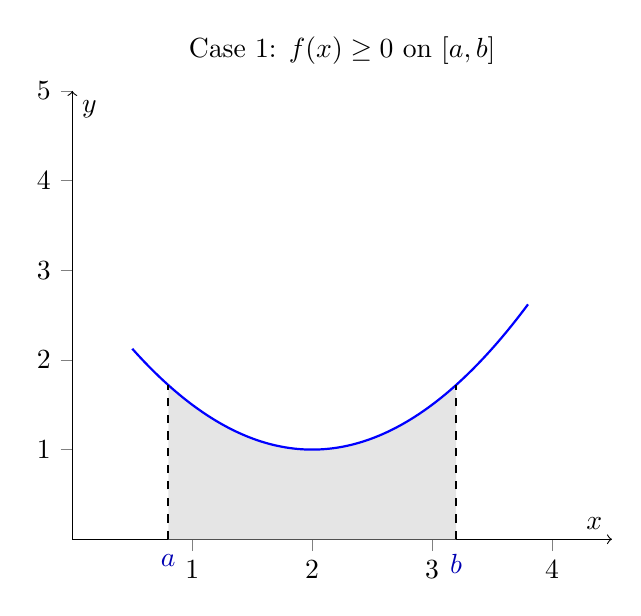
\begin{tikzpicture}
\begin{axis}[
  AreaAxisStyle,
  xmin=0, xmax=4.5,
  ymin=0, ymax=5,
  title={Case 1: $f(x)\ge 0$ on $[a,b]$}
]
  \def\a{0.8}
  \def\b{3.2}

  % Função f(x)
  \addplot[name path=curva, \CorCurvaSup, thick, domain=0.5:3.8, samples=200]
    {0.5*(x-2)^2+1};
  
  % Caminho invisível para o eixo X no intervalo [a,b]
  \addplot[name path=eixo, draw=none, domain=\a:\b] {0};

  % Preenchimento da área
  \addplot[\CorSombra] fill between[of=curva and eixo, soft clip={domain=\a:\b}];

  % Marcações a e b (calculando valores aproximados para f(a) e f(b))
  % f(0.8) = 1.72, f(3.2) = 1.72
  \MarcarAB{\a}{\b}{1.72}{1.72}
  
\end{axis}
\end{tikzpicture}
\caption{If $f(x)\ge 0$, then $A=\int_a^b f(x)\dif x$.}
\end{figure}

\end{document}
